
%\begin{figure}[t!]
%\begin{center}
%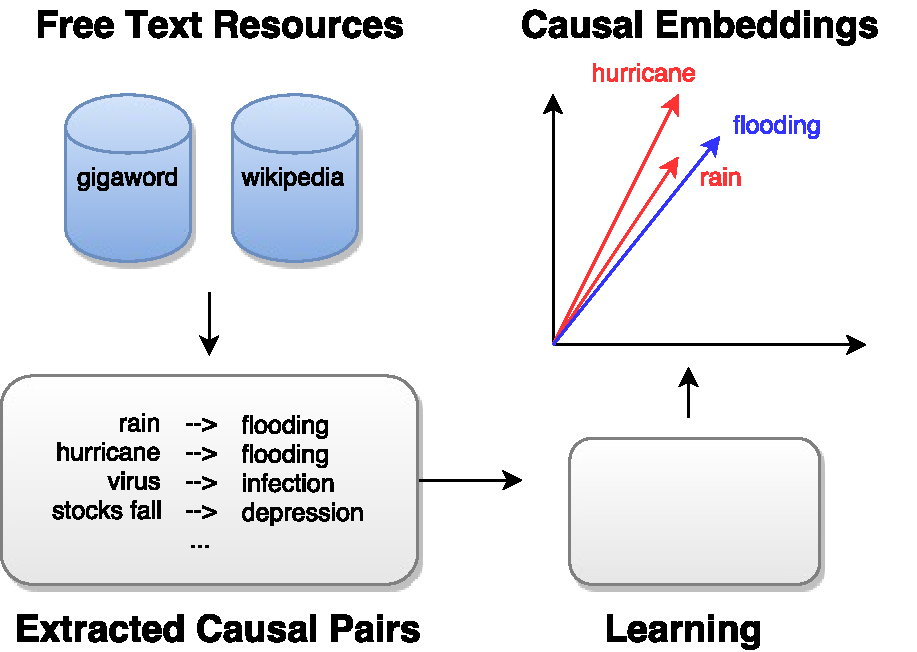
\includegraphics[width=75mm]{emnlpArchDraft.pdf}
%%\vspace{-4mm}
%\caption{{\small Our proposed pipeline for training a causal embedding space from free text resources. \todo{fill in learning with final model}}}
%\vspace{-6mm}
%\label{fig:arch}
%\end{center}
%\end{figure}
%
\section{Approach}
\label{sec:approach}
%\vspace{-2mm}

Our focus is on reranking answers to causal questions using using task-specific distributional similarity methods.
%on the the task of question answering, which is complicated by the variety of question types (e.g., definitional, causal),  each having different information needs that potentially require dedicated solving methods~\cite{clark2013study}.  
%Longer term, we propose a QA approach which uses dedicated, task-specific word embeddings for each question type, aimed at maintaining the robustness of word embeddings while gaining the specificity of dedicated solving methods. 
%Here, we address one particular information need: causality.
%
Our approach operates in three steps:

{\flushleft (1)} We start by bootstrapping a large number of cause-effect pairs from free text using a small number of syntactic and surface patterns (Section \ref{sec:causalextraction}).

{\flushleft (2)} We then use these bootstrapped pairs to build several task-specific embedding (and other distributional similarity) models (Section \ref{sec:models}). We evaluate these models directly on a causal-relation identification task (Section \ref{sec:directeval}).  

{\flushleft (3)} Finally, we incorporate these models into a reranking framework for causal QA and demonstrate that the resulting approach performs better than the reranker without these task-specific models, even if trained on the same data (Section ~\ref{sec:indirecteval}).  


%We approach the task of creating and evaluating a task-specific relational vector space by considering one relation in particular -- causality.  The architecture of our system is shown in Figure \ref{fig:arch}. \todo{do I really need an architecture here?}

%rule-based framework which analyzes free text and returns cause-effect tuples.  
%These pairs are then used to learn a set of high-dimensional word embeddings which are particular to the desired relation.  
%In particular, we make use of the Levy and Goldberg extension of the skipgram algorithm to learn embeddings from these pairs by predicting the effect-text given the cause-text.
%MOVE:
%using the extension of the Skipgram algorithm~\todo{cite and link} proposed by \citep{levy2014dependency}.  
%\todo{does this belong here? intro?}
%While the learning algorithm returns two distinct vector space embeddings for each item in the vocabulary, often only the target embeddings are ever used.  In this work, however, we make use of both sets of embeddings to capture the inherent \emph{directionality} of the causal relation.

%\todo{remove the evaluation info from here?}
%Once trained, we then evaluate the quality this mapping, or vector space, in two ways.  First, we evaluate it directly by attempting to rank a set of cause-effect pairs higher than entity pairs from other relations.  Second, we evaluate the mapping indirectly, by using it in the down-stream task of question answering (QA).

